\documentclass[11pt]{article}
\usepackage[margin=1in]{geometry}
\usepackage{amsmath,amssymb}
\usepackage{booktabs}
\usepackage{array}
\usepackage{graphicx}
\usepackage{hyperref}
\hypersetup{colorlinks=true,linkcolor=black,citecolor=black,urlcolor=blue}

\title{\textbf{End-to-End Project Workflow}\\[2pt]\large Detection and Attribution of AI-Generated and Human Written
Phishing Emails from Legitimate Emails Using Statistical Hypothesis Testing and Naive Bayes Classifiers}
\author{Mannan Bhardwaj -- 25BYB0013 \\ Bhoumik Singh Rajput -- 25BYB0120 \\[4pt]
School of Computer Science Engineering and Information Systems}
\date{}

\begin{document}
\maketitle

\section{Overview}
The project separates into two phases, run in sequence and never mixed: \textbf{Phase 1} happens once,
offline, on the labeled training corpus, and produces a fixed, locked set of statistically validated
features and model parameters. \textbf{Phase 2} happens per incoming email, at inference time, and only
ever applies the parameters Phase 1 already locked in -- it performs no further testing or fitting.
Figure~\ref{fig:pipeline} shows the full pipeline; the sections below walk through each stage in the
order the project actually executes them, including the stages already completed and the ones still
outstanding.

\begin{figure}[p]
\centering
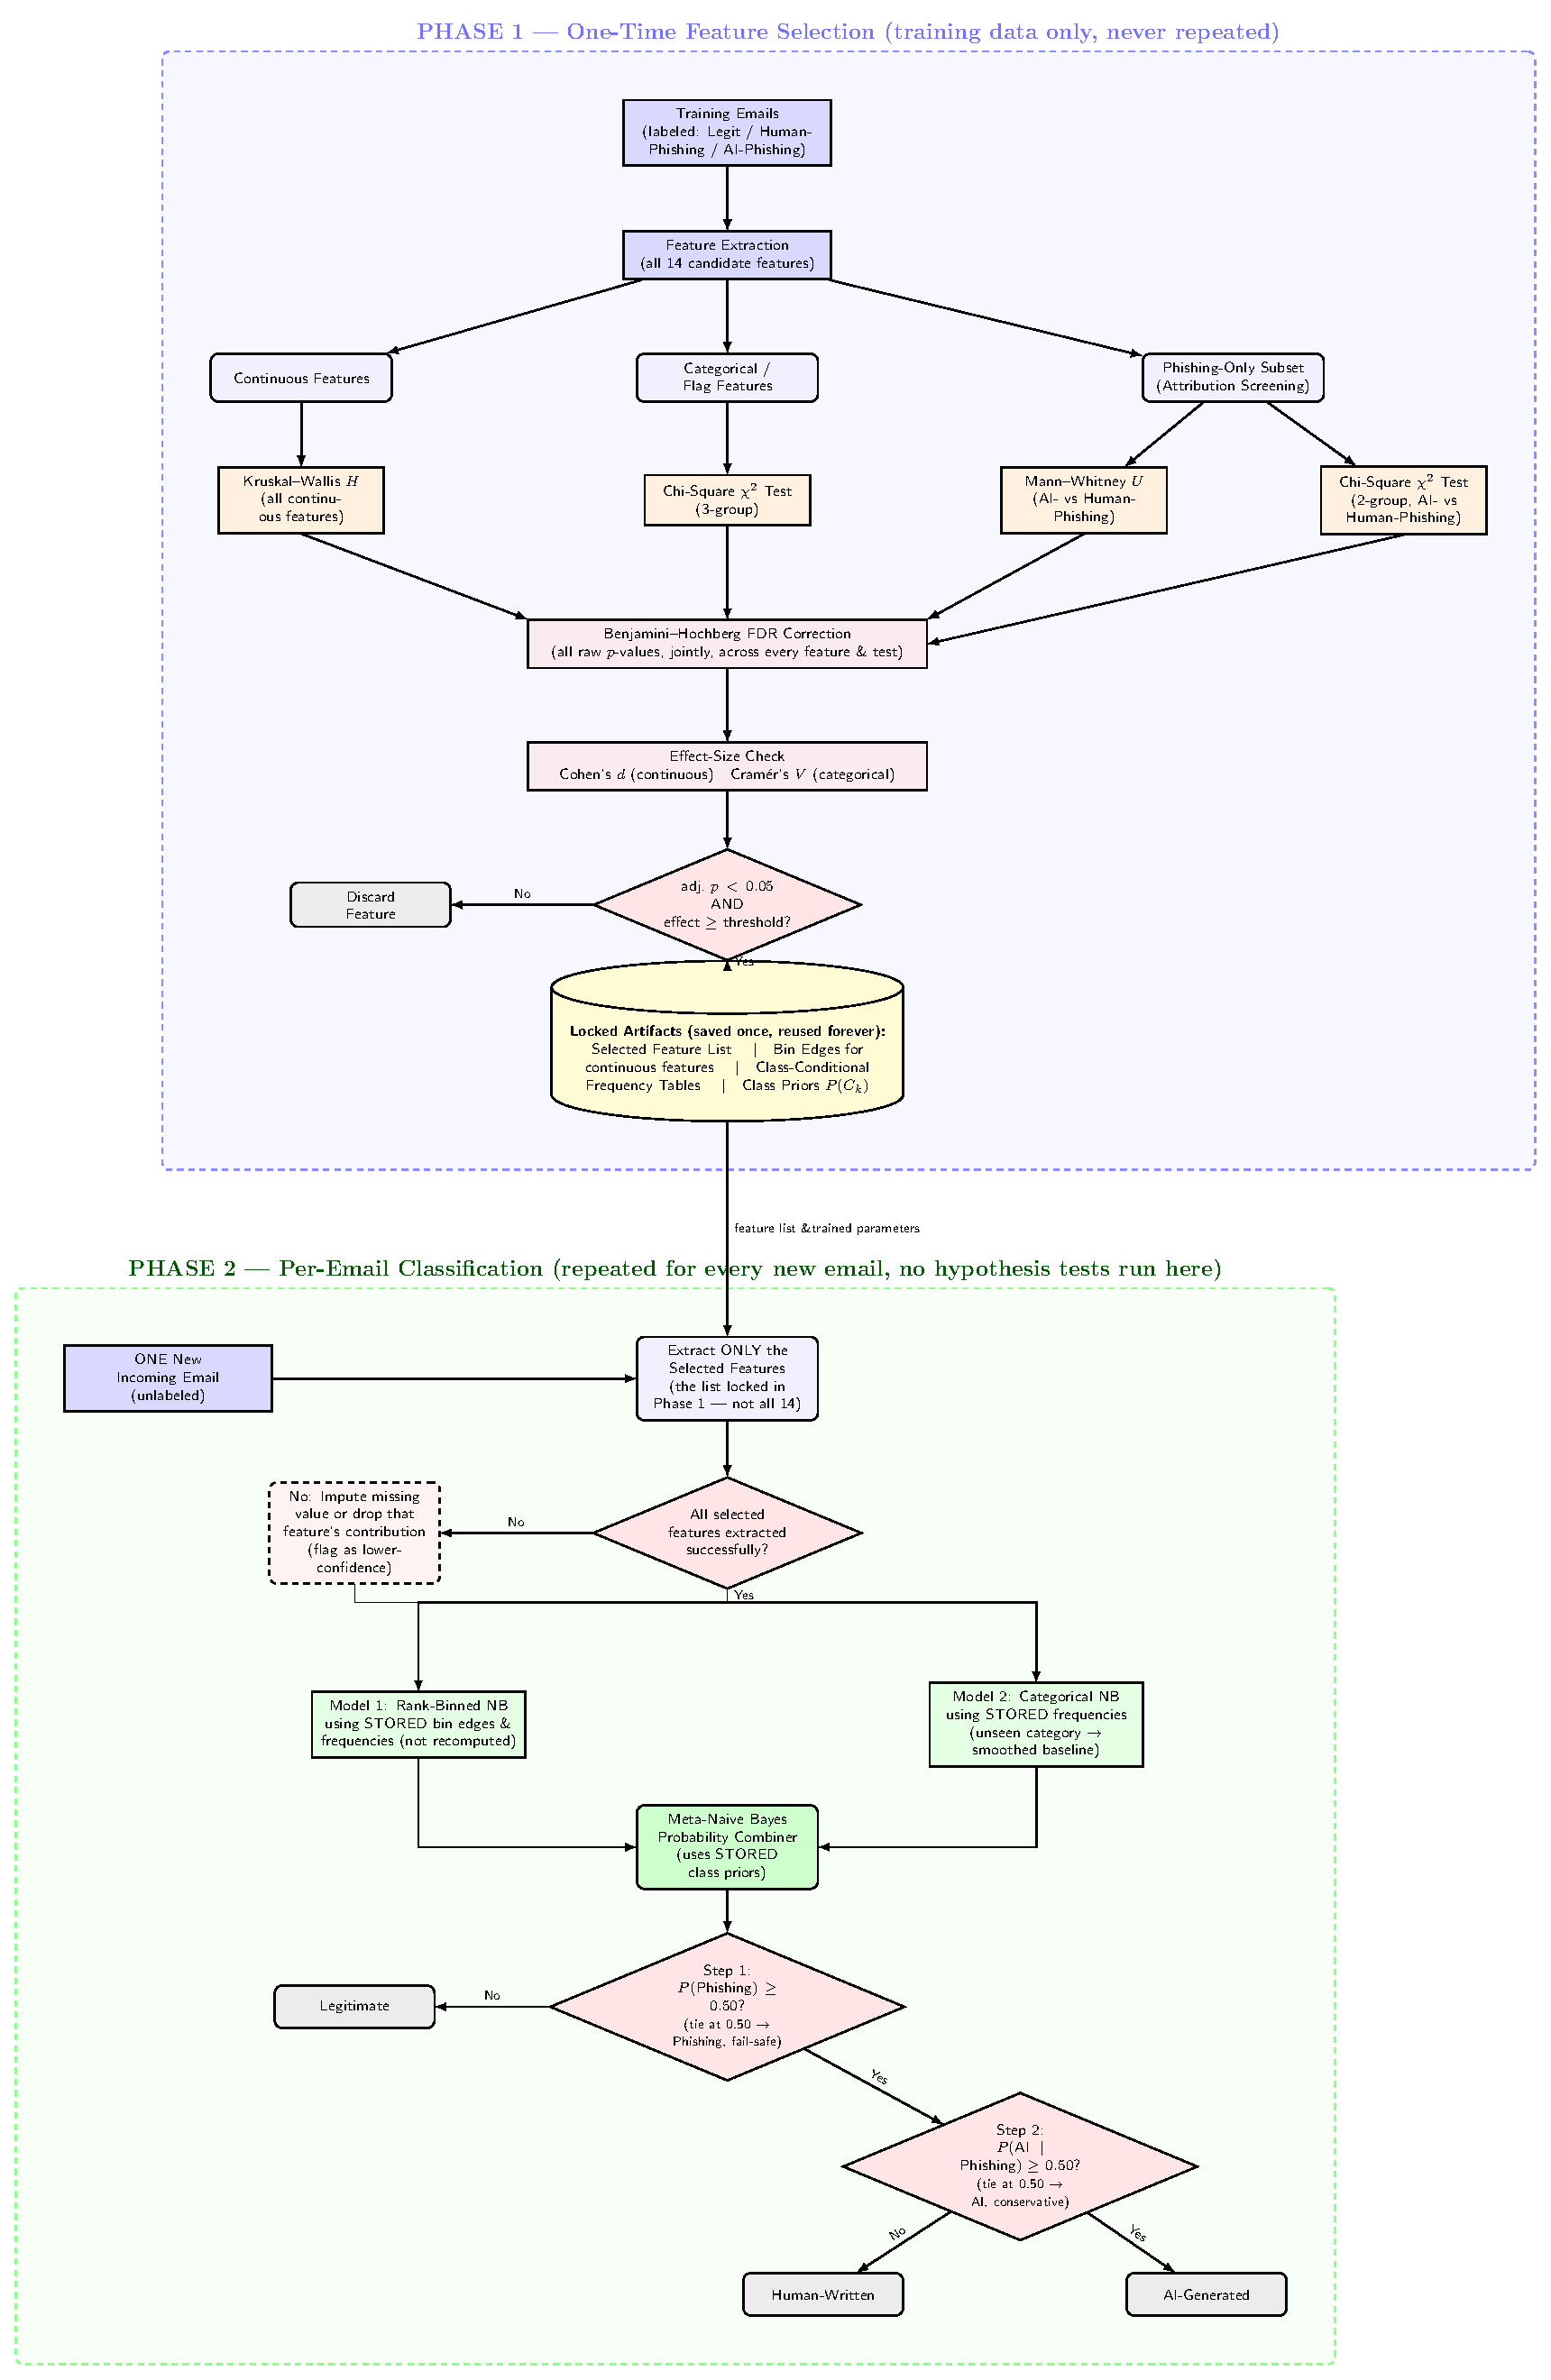
\includegraphics[width=\textwidth,height=0.92\textheight,keepaspectratio]{figure1_pipeline.pdf}
\caption{Two-phase pipeline: one-time feature selection (Phase 1) feeding locked parameters into
per-email classification (Phase 2).}
\label{fig:pipeline}
\end{figure}

\section{Stage 0: Data Acquisition and Cleaning \textit{(complete)}}
Three raw sources were combined into the three target classes:
\begin{itemize}
\item \textbf{Nazario\_5.csv} -- a real-world phishing corpus, source of both \textit{Legitimate} and
\textit{Human-Phishing} rows.
\item \textbf{emails\_sample\_5000.csv} -- a raw Enron sample, used as an independent, held-out
\textit{Legitimate} source to test generalization beyond Nazario's own legitimate mix.
\item \textbf{llm\_corpus\_sampled.csv} -- \textit{AI-Phishing} emails generated by three models
(GPT-4.1, DeepSeek 3.2, LLaMA 3.3 70B) across five pretexts (tax/IRS, HR, banking, parcel delivery,
IT support).
\end{itemize}
Cleaning removed 2 corrupted mbox-artifact rows, fixed a schema/label leak in Nazario's \texttt{urls}
column (re-derived URL counts directly from body text instead), removed empty-body rows, and
deduplicated the Enron and AI-Phishing pools. A corpus-collection artifact was also found and fixed: the
entire Nazario corpus was collected at one mailbox (\texttt{jose@monkey.org}), so that recipient identity
leaked into phishing-email text and had to be deleted (not placeholder-replaced -- an initial
placeholder-based fix was tried, found to relocate rather than remove the leak, and replaced) directly in
the dataset-building script.

\section{Stage 0.5: Dataset Validation \textit{(complete)}}
Two independent validation passes were run before the data was treated as trustworthy:
\begin{enumerate}
\item \textbf{Statistical/ML validity}: Kruskal-Wallis H-tests on ten quick proxy features (all
$p \approx 0$) and a TF-IDF + Logistic Regression baseline classifier (99.4\% cross-validated accuracy)
confirmed the three classes carry genuine, separable signal and let the top predictive tokens be
inspected directly to catch any remaining leakage.
\item \textbf{Bookkeeping/collision checks}: a separate workflow verifies the dataset's row-level
integrity independently of which features are used -- zero ID (hash) collisions, zero cross-class label
collisions (no email text labeled two different ways), zero train/holdout overlap, and near-duplicate
template reuse confined within single classes only. See the companion document,
\textit{Dataset Collision-Checking Workflow}, for the full methodology and current results.
\end{enumerate}
Output: \texttt{training\_set.csv} (4{,}491 rows, balanced 1{,}497/1{,}497/1{,}497 across Legitimate,
Human-Phishing, AI-Phishing) and \texttt{holdout\_set.csv} (8{,}465 rows, everything not used in
training).

\section{Phase 1, Stage 1: Feature Extraction \textit{(not yet started)}}
Twenty candidate features are computed for every email, split into two parallel tracks:
\begin{itemize}
\item \textbf{14 continuous features} across five categories -- Text Complexity and Predictability,
Structure and Syntax, Language Mechanics, Communication Style, and Lexical Richness (e.g.\ average token
log-probability, sentence-length standard deviation, punctuation entropy, urgency-keyword density,
lexical diversity).
\item \textbf{6 categorical/flag features} -- generic greeting, subject RE:/FW: marker,
attachment-mention, bracketed call-to-action, sensitive-info request, threat/consequence clause.
\end{itemize}
Full definitions and validation statistics for all 20 are in the companion document
\textit{Final Feature List}. This stage requires: a language-model scorer for token log-probability, a
syntactic parser for parse-tree depth, and a sentiment model for sentiment variance -- none of this
extraction code has been written yet; everything validated so far used hand-built proxy versions of a
subset of these features to confirm the approach works, not the final feature-extraction pipeline itself.

\section{Phase 1, Stage 2: Statistical Screening \textit{(proxy features validated; full 20-feature run pending)}}
Every continuous feature is tested with Kruskal-Wallis H (3-group) and, restricted to the phishing-only
subset, Mann-Whitney U (Human- vs AI-Phishing attribution). Every categorical feature is tested with
Chi-Square (3-group, and a 2-group attribution variant). All raw $p$-values from both tracks are
corrected jointly with Benjamini-Hochberg FDR, and a feature must also clear an effect-size floor
(Cohen's $d \geq 0.20$ continuous, Cram\'er's $V \geq 0.10$ categorical) to be retained. Only features
clearing both the significance and effect-size gates proceed to Stage 3. The 6 categorical features have
already been validated this way against real data (4 of 6 clear both gates for both tasks -- see the
\textit{Final Feature List} document for the full table); the 14 continuous features still need this run
performed against their real extracted values once Stage 1 exists.

\section{Phase 1, Stage 3: Parameter Locking \textit{(not yet started)}}
Whichever features survive Stage 2 have their class-conditional distributions (histogram bins for the
Rank-Binned NB, frequency tables for the Categorical NB) fit once on the training set and locked. No
further fitting happens after this point -- Phase 2 only ever applies these locked parameters.

\section{Phase 2: Per-Email Classification \textit{(not yet started)}}
For each new email: extract the locked feature set, then run two specialized Naive Bayes sub-models
independently -- a Rank-Binned NB over the continuous features and a Categorical NB over the categorical
features -- and combine their class-probability outputs through a Meta-Naive Bayes layer into one
posterior distribution. Classification proceeds in two steps: first Legitimate vs.\ Phishing, then, only
for emails flagged as phishing, Human-written vs.\ AI-generated attribution using the
attribution-validated feature subset. Ties at exactly $p=0.50$ follow an explicit tie-break rule rather
than an arbitrary default.

\section{Status Summary}
\renewcommand{\arraystretch}{1.3}
\begin{table}[h]
\centering
\begin{tabular}{@{}p{5.8cm}p{8.5cm}@{}}
\toprule
\textbf{Stage} & \textbf{Status} \\
\midrule
0. Data acquisition \& cleaning & Complete -- 3 sources merged, leak fixed, re-verified \\
0.5 Dataset validation (statistical + collision) & Complete \\
1.1 Feature extraction (20 features) & Not started -- needs LM scorer, parser, sentiment model \\
1.2 Statistical screening & Done for proxy/categorical features; full 20-feature run pending Stage 1.1 \\
1.3 Parameter locking & Not started \\
2. Per-email classification (NB sub-models + Meta-NB) & Not started \\
\bottomrule
\end{tabular}
\end{table}

The critical path forward is Stage 1.1: until the real feature-extraction code exists, every later stage
is blocked on it, and the statistical gate results currently documented for the 14 continuous features
remain provisional (computed on proxy features, not the final pipeline).

\end{document}
